\chapter{引论}
\label{chap:introduction}

\section{中微子}

中微子是标准模型中的一种基本粒子\cite{Griffiths:2008}。它拥有$1/2$的自旋特征,是一种费米子。中微子不带电,而且质量非常小,约在eV量级。
自然界中存在三种味道的中微子——电子中微子$\nu_e$,缪子中微子$\nu_\mu$和陶中微子$\nu_\tau$,他们分别对应于三种不同代的轻子——电子$e$,缪子$\mu$和陶子$\tau$。
在四种基本的相互作用中,中微子只参与引力相互作用和弱相互作用。

中微子的概念最早由泡利于1930年提出,当时泡利试图引入这种不带电的新粒子来解释贝塔衰变实验中能量不守恒的问题。
随后费米正式提出了一套关于电弱相互作用的理论模型,即费米四顶点模型,其中便包含了泡利提出的不带电的新粒子。
如果这个新粒子的质量非常小,那么贝塔衰变中观测到的电子能谱便能够被非常完美地解释。
因此费米称这个新粒子为中微子(neutrino,在意大利语中意味着中性的微小粒子)。

自弱相互作用模型和中微子被提出以来,中微子便成为了粒子物理领域的一大研究热点。
1941年,我国核物理学家王淦昌首次提出了用贝塔捕获的方式来探测中微子\cite{Wang:1942}。
1956年, Clyde Cowan和Frederick Reines等人通过反贝塔衰变的方式首次真正探测到了中微子的存在\cite{Cowan:1956}。他们也因此在约40年后被授予1995年的诺贝尔物理学奖。

\begin{figure}[htb]
    \centering
    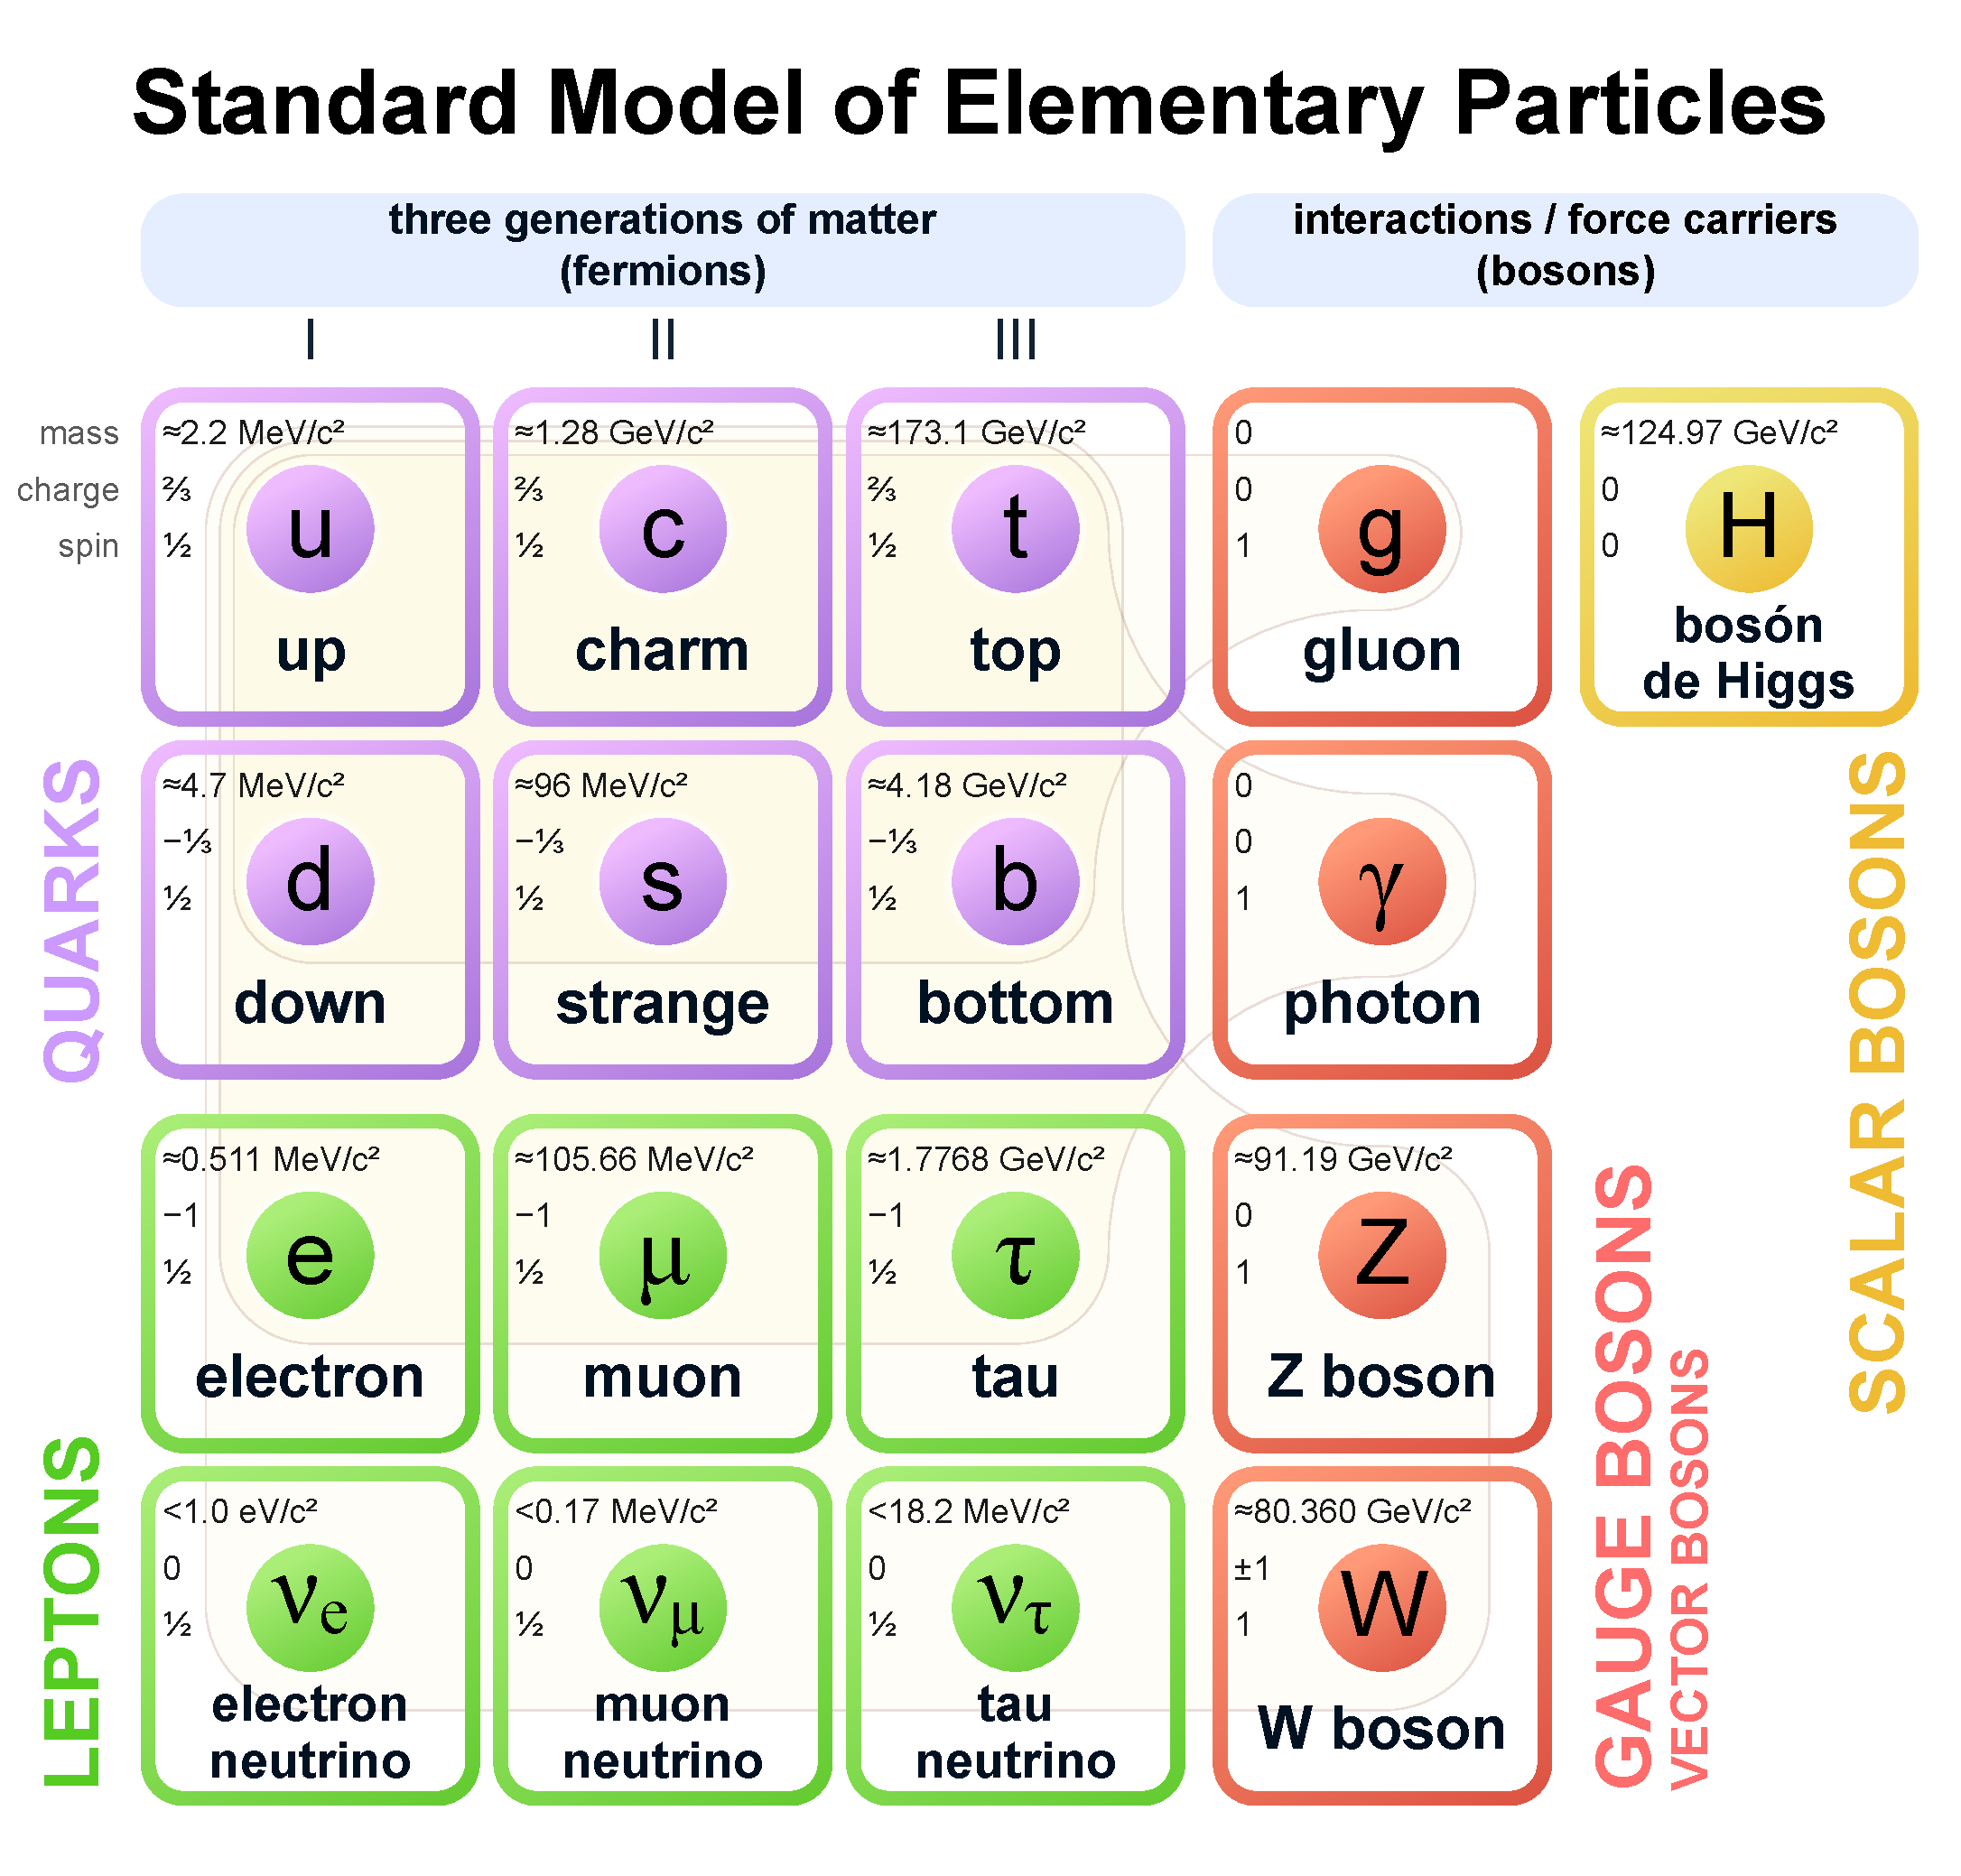
\includegraphics[width=0.8\linewidth]{img/standard_model.pdf}
    \caption{粒子物理标准模型中粒子以及假设的引力子。图片来自于维基百科}
    \label{fig:standard_model}
\end{figure}

\subsection{中微子振荡}

自19世纪50年代以来,Raymond Davis便已经在进行有关太阳中微子的探测\cite{Davis:1955}。在经过了数十年的实验后,他终于测到了太阳中微子,并因此获得了2002年的诺贝尔物理学奖。但与此同时,他在实验中也发现了太阳中微子的流量要低于理论预期值\cite{Cleveland:1998},这个问题被称为“太阳中微子缺失问题”。

中微子振荡模型可以用于解释“太阳中微子缺失问题”\cite{Bahcall:2001}。标准模型并没有限制中微子必须是无质量粒子,假如中微子存在质量的话,那么它的质量本征态($|\nu_k\rangle$,其中$k=1,2,3$),可以构成与味道本征态($ |\nu_\alpha\rangle$,其中$\alpha = e, \mu, \tau$)相互独立的一组量子态基矢,我们观测到的味道本征态的中微子可以是由不同的质量本征态的中微子相互组合后产生的:
\begin{equation}
    \left|v_{\alpha}\right\rangle = \sum_{k=1}^{3} U_{\alpha k}^{*}\left|v_{k}\right\rangle , 
    \label{eq: neutrino oscillation}
\end{equation}
其中$U$是一个幺正矩阵,被称作轻子混合矩阵,或者Pontecorvo-Maki-Nakagawa-Sakata (PMNS)矩阵\cite{Pontecorvo:1957, Maki:1962, Pontecorvo:1967}。它通常被分解成如下的形式:
\begin{equation}
    U=\left(\begin{array}{ccc}{1} & {0} & {0} \\ {0} & {c_{23}} & {s_{23}} \\ {0} & {-s_{23}} & {c_{23}}\end{array}\right)\left(\begin{array}{ccc}{c_{13}} & {0} & {s_{13} e^{-i \delta_{\mathrm{CP}}}} \\ {0} & {1} & {0} \\ {-s_{13} e^{i \delta_{\mathrm{CP}}}} & {0} & {c_{13}}\end{array}\right)\left(\begin{array}{ccc}{c_{12}} & {s_{12}} & {0} \\ {-s_{12}} & {c_{12}} & {0} \\ {0} & {0} & {1}\end{array}\right) P_\nu , 
    \label{eq: PMNS matrix}
\end{equation}
其中$c_{ij}$和$s_{ij}$分别表示中微子振荡角$\theta_{ij}$的余弦值和正弦值,$\delta$表示狄拉克CP对称性破坏相位角,而$P_\nu = \mathrm{Diag} \{e^{i\rho},  e^{i\sigma}, 1 \}$表示马约拉纳相位角并与中微子振荡现象无关。

中微子振荡现象最终在超极神冈(Super-Kamiokande)和Sudbury中微子观测站中得到了验证\cite{Super-K:1998, Sudbury:2001}。
中微子振荡被认为是人们发现的首个超出标准模型的物理现象。2015年的诺贝尔物理学奖授予Takaaki Kajita和Arthur B. McDonald,以此来表彰他们在中微子振荡中做出的贡献。


\subsection{无中微子双贝塔衰变}

马约拉纳粒子是一种反粒子便为自身的费米子。这种粒子的概念由Ettore Majorana于1937提出。
由于马约拉纳粒子必须不带有电荷,因而中微子便成为了标准模型框架下唯一可能的马约拉纳粒子。
假如中微子真的是马约拉纳粒子,那么它将破坏轻子守恒定律,而这通常是超出标准模型的新物理的特征。
然而中微子微小的质量使得我们难以确认它到底是狄拉克粒子还是马约拉纳粒子。

目前实验上确认中微子是否是马约拉纳粒子的唯一途径便是观测无中微子双贝塔衰变($0\nu\beta\beta$):
\begin{equation}
    N(A, Z) \rightarrow N(A, Z+2) +2 e^{-} ,
    \label{eq: double beta decay}
\end{equation}
其中$N(A, Z)$表示质子数和中子数都为偶数的原子核,且它的质量必须大于与之拥有同样中子数但大两个质子数的原子核$N(A, Z+2)$。满足该特征的原子核有$^{48}Ca$,$^{76}Ge$和$^{136}Xe$等。
目前已经有许多项正在进行和规划中的实验来探寻$0\nu\beta\beta$信号,例如:PandaX\cite{PandaX-II:2019},KamLAND-Zen\cite{KamLAND-Zen:2016},EXO-200\cite{EXO-200:2012}等等。$0\nu\beta\beta$实验被认为是寻找新物理的重要方向。


\section{高能中微子天文学}

由于具有不带电且相互作用微弱的性质,中微子可以穿越复杂的宇宙环境而到达地球,是一种观测宇宙的重要信使。用中微子来观测宇宙中的物理现象,这便是中微子天文学。
通过中微子信使,人们可以观测到天体中光子无法穿透的高密度区域。中微子天文学在粒子物理,天体物理以及宇宙学中都有重要的作用。
例如,太阳中微子的观测对于理解太阳内部的核反应过程和建立标准太阳模型有至关重要的作用\cite{Bahcall_solar_model:2005}。
在1987年,人们在银河系的卫星星系——大麦哲伦星云中发生的超新星爆发SN 1987a中探测到了中微子\cite{Hirata_sn:1987, Bionta_sn:1987}。这为超新星爆发模型提供了有力的支持,该模型认为超新星中的大部分能量都以中微子的形式释放了出去。
本文的主要研究对象为高能中微子(亚TeV-EeV能级),故在下文中我们主要讨论天体物理起源的高能中微子,并且在不做特殊说明的情况下,我们在后文中将高能中微子天文学简称为中微子天文学。

\subsection{高能宇宙线与中微子}

\subsubsection{高能宇宙线简介}

宇宙线是来自宇宙中的高能带电粒子,它的成分主要是质子和少量的氦核以及其他重核\cite{Gaisser:2016}。
宇宙线的能量可以跨越数个量级,从$\sim 10 \,\mathrm{GeV}$一直延续到$\sim 100 \,\mathrm{EeV}$,其高能段远远超过了人类目前制造的加速器所能加速能量的极限。
宇宙线的能谱如图\ref{fig:CR_spectrum}所示,呈现幂律谱的形式:在低能处数量较多,例如在$\sim 1 \,\mathrm{TeV}$处每平方米每秒就会有一个宇宙线粒子通过,而高能处事例数极少,例如在$\sim 100 \,\mathrm{PeV}$处大约每平方米每年才会有一个宇宙线粒子通过。
自上世纪30年代宇宙线被人类发现以来,人们通过宇宙线发现了大量新的粒子,例如$\pi$介子,缪子,K介子等。
尽管人们对宇宙射线的研究在近百年的时间内从未停止过,超高能宇宙线粒子的起源至今没有明确的答案。
这是由于宇宙线携带电荷,它在星际传播的过程中受到磁场的影响而改变其传播方向,因此人们在地球上难以从观测到的宇宙线追溯回它来源的天体。
相比之下,中微子不带电且相互作用微弱,探测与高能宇宙线同时产生的高能中微子将有助于解答高能宇宙线起源的百年难题。

\begin{figure}[htb]
    \centering
    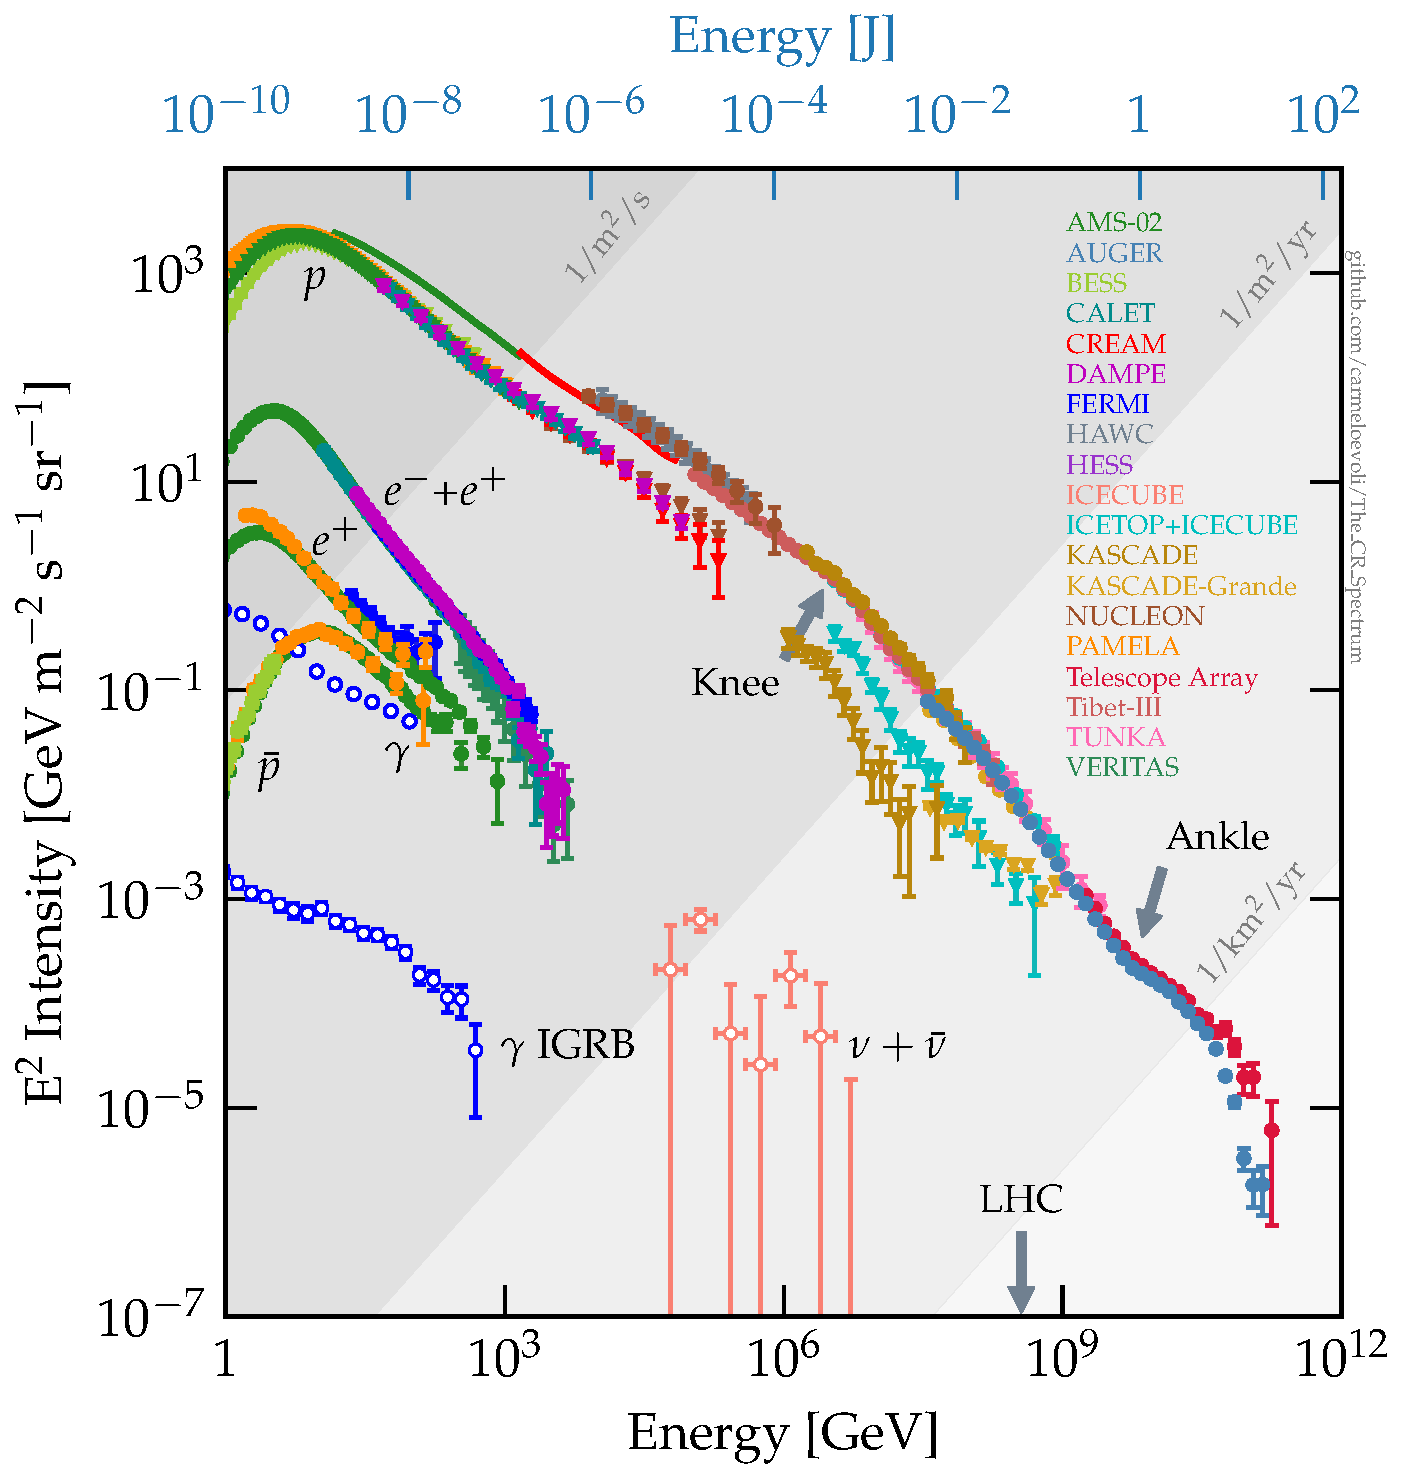
\includegraphics[width=0.8\linewidth]{img/cosmic_ray_spectrum.pdf}
    \caption{各个成分的宇宙线的流量随着能量的变化关系。图片来自\cite{CR_spectrum:2022}}
    \label{fig:CR_spectrum}
\end{figure}

\subsubsection{宇宙线加速机制}

宇宙线能谱的幂律形式可以用费米加速机制来解释。费米曾经提出了一种加速机制,即利用一团运动的磁云来多次使得粒子在其中来回地被磁场弯曲弹射\cite{Fermi_acceleration:1949},其物理图像如图\ref{fig:CR_acceration}中左图所示。
宇宙线粒子在每一次与磁云的碰撞过程(即受到磁云的磁场的作用而改变运动方向)中,粒子都会获得正比于自身初始能量的能量。因此,在经过多次碰撞后,粒子将获得极高的能量。
并且,粒子在每次碰撞过程中都有一定几率摆脱磁云的束缚而离开加速区,进而被地球的观测者所观测到。在这两种效应的结合下,最终观测者看到的粒子能谱会呈现出观测到的幂律谱的形式。

费米加速机制可以很好地解释观测到的幂律能谱,它在后续的几年中被不断地改进,并且应用到大量其他的天体物理环境中,其中最著名的便是扩散激波加速机制\cite{Bell_shock_1:1978, Bell_shock_2:1978},其图像如图\ref{fig:CR_acceration}中右图所示。
在扩散激波加速机制中,粒子每次碰撞所获得的能量正比于激波速度$v/c$的一次方,而非原始费米加速机制下的二次方,因而具有更高的加速效率。根据加速过程中获得能量与激波速度的幂律关系,扩散激波加速机制也被称为一阶费米加速机制,而通过磁云碰撞的加速机制则被称为二阶费米加速机制。

\begin{figure}[htb]
    \centering
    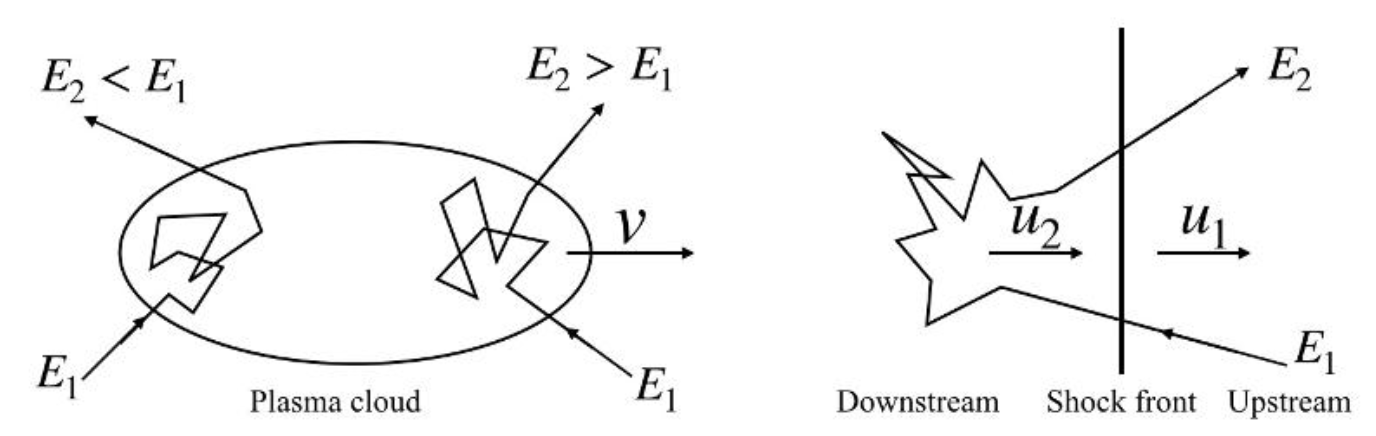
\includegraphics[width=0.8\linewidth]{img/Fermi_acceleration.png}
    \caption{宇宙线加速的模型。左图:费米二阶加速机制。宇宙线粒子与等离子体磁云碰撞而获得能量;右图:费米一阶加速机制,等离子体来回穿过激波上下游而获得能量。图片来自\cite{Gaisser:2016}}
    \label{fig:CR_acceration}
\end{figure}

在天体物理环境下,磁场的能量密度通常比较高,因此磁场可以使得带电粒子被束缚在加速区域中,从而有可能通过多次发生碰撞的形式得到加速。在这种图像下,带电粒子的能量不应过高,否则其回旋半径将会超过加速区的大小从而离开。磁场束缚下带电粒子加速的能量极限$E_\mathrm{Hillas}$被称为Hillas极限\cite{Hillas_limit:1984}:
\begin{equation}
    E_\mathrm{Hillas} = Z e c B R ,
\end{equation}
其中$Z$为带电粒子电荷数,$e$为元电荷量,$c$为光速,$B$和$R$分别为加速区的磁场大小和半径大小。

目前我们已经观测到$\sim 100\,\mathrm{EeV}$的宇宙线,即便是如此高的能量,依然有许多天体物理源的环境能够满足Hillas条件\ref{fig:Hillas_limit}。
他们中有的是具有极端的磁场环境,例如磁性,脉冲星和白矮星;有的是具有天体物理尺度的体积,例如射电星系和星系团。
对高能天体中微子的探测能够帮助我们定位究竟是何种天体源能够将粒子加速到如此高的能量,从而为理解具体的天体物理现象和宇宙线加速机制提供帮助。

\begin{figure}[htb]
    \centering
    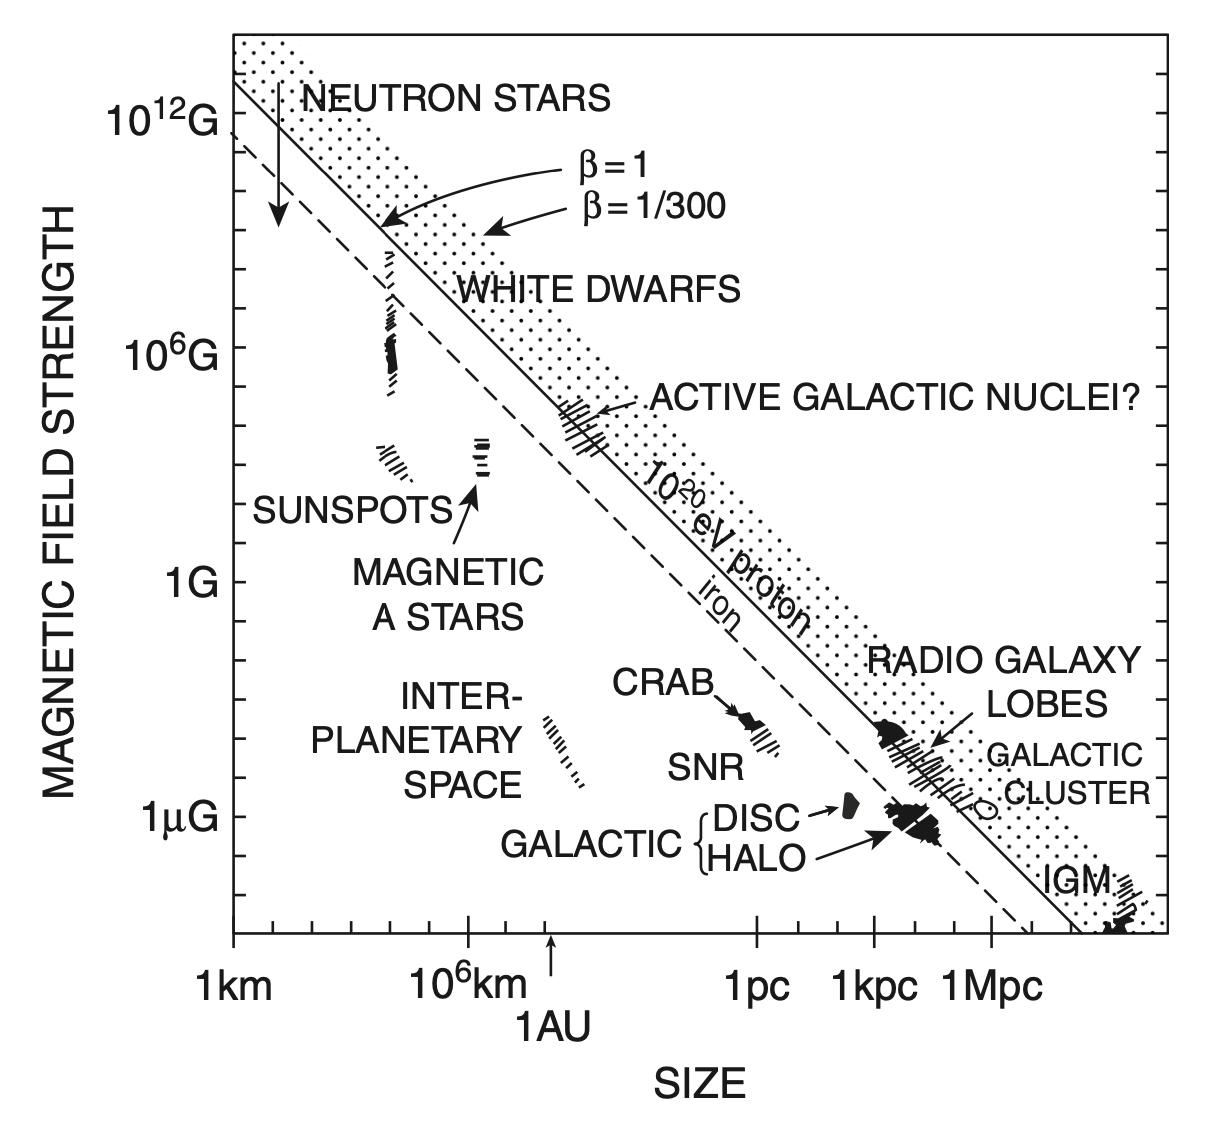
\includegraphics[width=0.8\linewidth]{img/Hillas_limit.png}
    \caption{潜在的宇宙线起源天体以及它们的大小和磁场强度。源的大小与磁场强度的乘积决定了源能加速的宇宙线的上限,即Hillas条件。图片来自\cite{Gaisser:2016}}
    \label{fig:Hillas_limit}
\end{figure}

\subsubsection{高能中微子产生机制}
\label{subsubsec:neutrino_production}

由于中微子不带电荷,故中微子自身难以被加速。在天体物理环境下,高能中微子主要由高能宇宙线粒子与其他粒子碰撞产生。
宇宙线粒子和重子背景或者光子背景碰撞,产生$\pi$介子,$K$介子等次级粒子,这些次级粒子通过衰变产生中微子。

以宇宙线中的质子为例,$pp$过程中质子与质子的非弹性散射表达式如下:
\begin{equation}
    p+p \rightarrow M_{p p}^{+} \pi^{+}+M_{p p}^{-} \pi^{-}+M_{p p}^0 \pi^0 + X ,
    \label{eq:pp_interaction}
\end{equation}
其中$M_{p p}^{+}: M_{p p}^{-}: M_{p p}^0 \approx 1: 1: 1$表示反应中产生的$\pi^{+}$,$\pi^{-}$和$\pi^{0}$粒子的数量,$X$表示其他更高阶的强子产物,例如$K$介子和$\Lambda$介子等。

另外一种反应通道——$p\gamma$过程中质子与光子的共振散射表达式如下:
\begin{equation}
    p+\gamma \rightarrow \Delta^{+} 
    \rightarrow\left\{
    \begin{array}{l}
        n+\pi^{+} \\
        p+\pi^0
    \end{array}
    \right. ,
    \label{eq:pgamma_interaction}
\end{equation}
其中$\Delta^{+}$是质子的共振态,拥有更高的质量和自旋,它会快速地通过强相互作用衰变为强子和$\pi$介子,衰变为中子和质子的几率比为$1/3 : 2/3$。

无论是$pp$过程还是$p\gamma$过程,单个产生的$\pi$介子从初始的高能质子中继承来的能量比例都约为:
\begin{equation}
    x_\pi = \left \langle \frac{E_\pi}{E_p} \right \rangle \simeq 0.2 ,
\end{equation}
其中$E_p$是高能质子的能量,$E_\pi$是反应产生的$\pi$介子的能量。

以上两种反应中产生的$\pi$介子会继续通过电弱相互作用衰变,产生中微子和光子:
\begin{equation}
    \begin{aligned}
        & \pi^{+} \rightarrow \mu^{+}+v_\mu \rightarrow e^{+}+v_e+\bar{v}_\mu+v_\mu \\
        & \pi^{-} \rightarrow \mu^{-}+\bar{v}_\mu \rightarrow e^{-}+\bar{v}_e+v_\mu+\bar{v}_\mu \\
        & \pi^0 \rightarrow 2 \gamma ,
        \label{eq:pion_decay}
    \end{aligned}
\end{equation}
在衰变过程中,我们可以近似地认为衰变产生的2个伽马光子各自携带$\pi$介子$1/2$的能量,4个轻子各自携带$\pi$介子$1/4$的能量。
因此最终反应得到的中微子的能量约为初始质子能量的$5\%$,光子的能量约为初始质子能量的$10\%$。

值得注意的是,由于缪子的寿命($2.2\,\mathrm{\mu s}$)要远远大于$\pi$介子的寿命($26\,\mathrm{ns}$),在部分强磁场的天体物理环境下,缪子可能会经历显著的能损过程,导致最终发生衰变时,其能量已经远低于初始能量,故缪子衰变得到的中微子可以忽略不计\cite{muon_damp:2005}。
在这种情况下,天体物理源处的各个中微子味道的比例将会从公式\ref{eq:pion_decay}中所描述的$v_e: v_\mu: v_\tau \approx 1: 2: 0$转变为$v_e: v_\mu: v_\tau \approx 0: 1: 0$。

目前对弥散的宇宙线流量,中微子流量,和伽马光子流量的观测如图\ref{fig:diffuse_neutrino_CR_gamma}所示,三种不同的信使之间存在着能量区间和流量大小的差异。
我们可以看到弥散伽马射线在高能处存在截断,这是由于极高能($\gtrsim 1\,\mathrm{TeV}$)的光子可以与星系间的背景光子场发生作用而产生正负电子对,因此宇宙对极高能的光子是不透明的。
宇宙线只画了GeV到EeV的能级,这是因为更低能量的宇宙线粒子在星际间磁场的作用下,其运动行为接近随机游走,已经彻底丧失了方向性。而更高能处宇宙线粒子的流量截断是由GZK效应,即宇宙线与宇宙微波背景辐射相作用导致的\cite{GZK_G:1966, GZK_ZK:1966}。

\begin{figure}[htb]
    \centering
    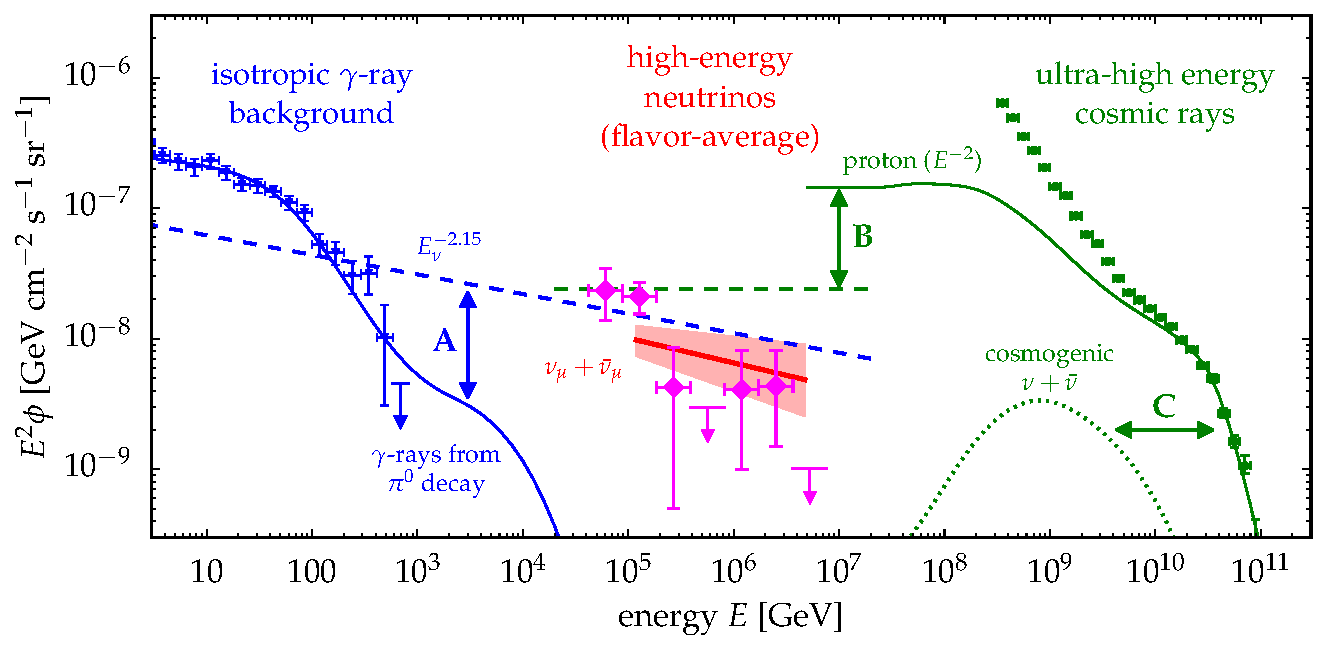
\includegraphics[width=0.8\linewidth]{img/diffuse_neutrino_CR_gamma.pdf}
    \caption{IceCube观测到的弥散中微子能谱(红色线表示缪子径迹事件的分析结果\cite{IceCube_diffse_muon:2017},粉色数据点表示高能起始事件的分析结果\cite{IceCube_6yr_cascade_spectrum:2017}),Fermi-LAT观测到的弥散的银河外伽马射线能谱(蓝色数据点)\cite{Fermi_diffuse_gamma:2014},以及Auger观测到的极高能宇宙线能谱(绿色数据点)\cite{Auger_diffuse:2015}。图片来自\cite{Astro2020_neutrino}}
    \label{fig:diffuse_neutrino_CR_gamma}
\end{figure}


\subsection{天体中微子源}

宇宙中有许多剧烈活动的天体,它们中有的已经被观察到了强烈的伽马射线辐射,表明他们具备加速宇宙线粒子的能力。
这些天体在加速宇宙线的过程中,如果能够将质子加速到超过PeV能级,并且在加速区域附件的背景场中存在足够多的气体或者光子成分,那么便有可能产生高能的中微子辐射。
在下面内容中,我们列举一些有潜力的高能中微子的天体源,如果想要了解更详细的研究,读者可以参考最近的综述\cite{Kurahashi_review_nu_mm:2022}。这些天体源有的是灾变型事件,具有比较短的活动时间,因而被称为暂现源,有的可以在上千年的时间中稳定地产生中微子,因而被称为持续源。

\subsubsection{暂现源}

伽马射线暴(Gamma Ray Burst,GRB)是自宇宙大爆炸之后最剧烈的天体活动之一,它能够在$\sim 1\,\mathrm{s}$的时间尺度上释放出$10^{51}-10^{53}\,\mathrm{erg}$能量的光子\cite{zhang:2018}。宇宙中的GRB事件所释放出来的能量足以产生我们所观测到的极高能宇宙线流量,是非常有潜力的极高能宇宙线的起源天体\cite{Waxman:1995}。此外,MAGIC和LHAASO分别在GRB 190114C和GRB 221009A中观测到了高达TeV能级的伽马光子\cite{MAGIC_GRB190114C:2019},证实了其高效的加速粒子能力。因此,GRB一直以来都被认为是非常有潜力的中微子源\cite{Waxman:1997ti}。

潮汐瓦解事件(Tidal Disruption Event,TDE)是恒星被超大质量黑洞吞噬时产生的事件。观测和数值模拟表明,TDE中可能包含有吸积盘,半相对论性的物质流出(outflow),以及可能包含一个喷流(jet)\cite{Dai_TDE:2018}。物质流出和喷流的结构可以将强子加速到高能,而吸积盘则可以提供背景光子场,因此TDE具备产生高能中微子的潜力\cite{Wu_TDE:2021, Zheng_TDE:2022, Winter_TDE:2022}。

\subsubsection{持续源}

脉冲星风星云(Pulsar Wind Nebulae,PWN)是由中子星向外发射的相对论性的星风与周围的介质相互作用产生的结构\cite{Mitchell_PWN:2022}。
PWN可以产生从射电到伽马射线的广谱辐射,最近LHAASO的观测表明脉冲星风星云可以产生PeV能量的伽马光子辐射\cite{LHAASO_Crab:2021},预示着PWN有能力将带电粒子加速到大于PeV的能量。

星爆星系(starburst galaxy)是指存在着高密度的气体,恒星形成活跃的星系。星爆星系中大质量恒星晚期的灾变事件发生频繁,具有充足的宇宙线供应。而且恒星会产生较强的磁场环境,将宇宙线束缚在其中,导致$\lesssim 1\,\mathrm{PeV}$的宇宙线与气体碰撞的时标要短于逃离时标,因此具备产生高能的弥散中微子流的潜力\cite{Loeb_starburst_galaxy:2006}。

活动星系核(Active Galactic Nuclei,AGN)是一个正在吸积物质的星系中心超大质量黑洞,在黑洞的附近存在着很强的紫外射线和X射线的辐射场。黑洞吸积盘中的物质在落入黑洞时,可能会和光子场发生作用,从而通过$p\gamma$过程产生中微子辐射\cite{Meszaros_AGN:2004, Murase_AGN:2015, Murase_AGN:2022, Murase_hidden_AGN:2022}。


\subsection{IceCube观测结果}

IceCube是目前世界上正在运行中的最大的中微子望远镜,它取得了丰富的观测结果。IceCube于2013年首次发现了来自宇宙中的高能中微子存在的证据\cite{IceCube_astro_neutrino_flux:2013}。2014年,IceCube又以$5.4\sigma$的置信度确认了它的存在\cite{IceCube_astro_neutrino_flux_3yr:2014},至此,IceCube宣布了高能天体物理中微子天文学的研究正式开始。

\subsubsection{弥散中微子能谱}

IceCube每年大约能观测到$\mathcal{O}(10)$个能量大于$100\,\mathrm{TeV}$的中微子事件。相比于大气缪子和大气中微子背景,这些高能的事件极有可能来自地球以外的宇宙空间中。
这些中微子事件在时间和空间上呈现出全天各向同性的分布,并没有明显地和已知的天体物理源成协。
通过对中微子事件进行筛选分析,IceCube测量出了弥散天体物理中微子能谱\cite{IceCube_6yr_cascade_spectrum:2020, IceCube_HESE:2020, IceCube_MESE:2014, IceCube_diffse_muon:2021, IceCube_starting_track:2021b}。不同分析的测量结果如图\ref{fig:IceCube_diffuse_spectrum}所示,图中的横坐标$\gamma_\mathrm{astro}$和纵坐标$\phi^{\nu_i+\bar{\nu}_i}_\mathrm{astro}$分别表示某一种味道的中微子能谱的谱指数和在$100\,\mathrm{TeV}$下的流量大小,即中微子能谱被表示为幂律谱的形式:
\begin{equation}
    \phi^{\nu_i+\bar{\nu}_i}_\mathrm{astro}(E_\nu) = \phi^{\nu_i+\bar{\nu}_i}_\mathrm{astro, 100\,TeV} \times \left( \frac{E_\nu}{100\,\mathrm{TeV}} \right)^{-\gamma_\mathrm{astro}} \times 10^{-18} \, \mathrm{s^{-1} cm^{-2} GeV^{-1} sr^{-1}}
    \label{eq:diffse_nu_flux}
\end{equation}

我们可以看到在图\ref{fig:IceCube_diffuse_spectrum}中,不同的筛选条件得到的样本的能谱略有差异,由能量阈值最低的来自北天的径迹型事件\cite{IceCube_diffse_muon:2021}测量得到的能谱比较硬,能量阈值中等的簇射型事件\cite{IceCube_MESE:2014, IceCube_6yr_cascade_spectrum:2020}测出的能谱比较软,而高能簇射型事件\cite{IceCube_HESE:2020}得到的能谱最软,其值接近-3。
这可能预示着中微子的能谱从低能到高能可能存在着由硬逐渐变软的过程,而并非一个单一的幂律谱。

\begin{figure}[htbp]
    \centering
    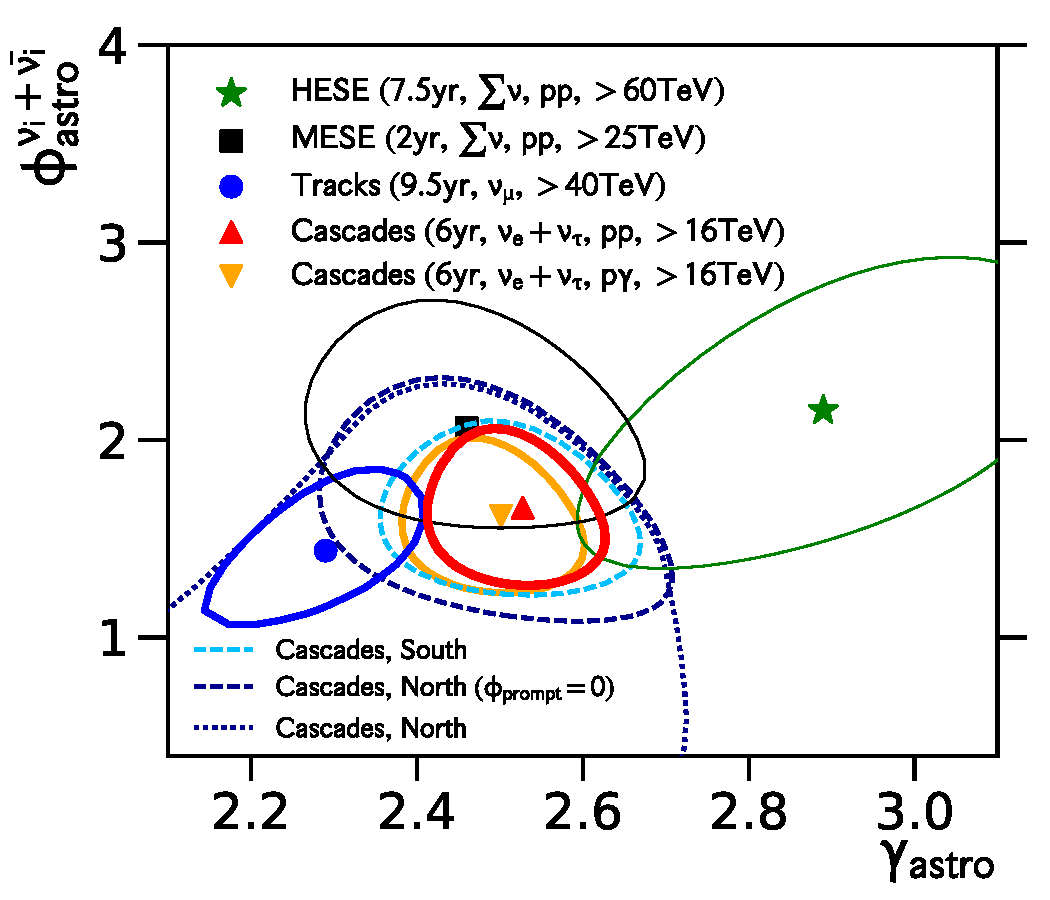
\includegraphics[width=0.6\linewidth]{img/IceCube_diffuse_spectrum.pdf}
    \caption{IceCube筛选不同的数据集测量得到的弥散中微子能谱。图片来自\cite{IceCube_6yr_cascade_spectrum:2020}}
    \label{fig:IceCube_diffuse_spectrum}
\end{figure}

IceCube通过对弥散中微子流量的数据分析表明中微子源呈现出单个源流量弱而数量多的弥散特征,因此整体上源的搜寻比较困难。IceCube对源的密度和亮度的限制如图\ref{fig:neutrino_sources}所示。
这种数量弥散而亮度微弱的源要求下一代的中微子望远镜必须具备更好的角分辨率和有效面积,才能从弥散的流量中寻找到确切的中微子源\cite{Fang_resolve_flux:2016}。

\begin{figure}[htbp]
    \centering
    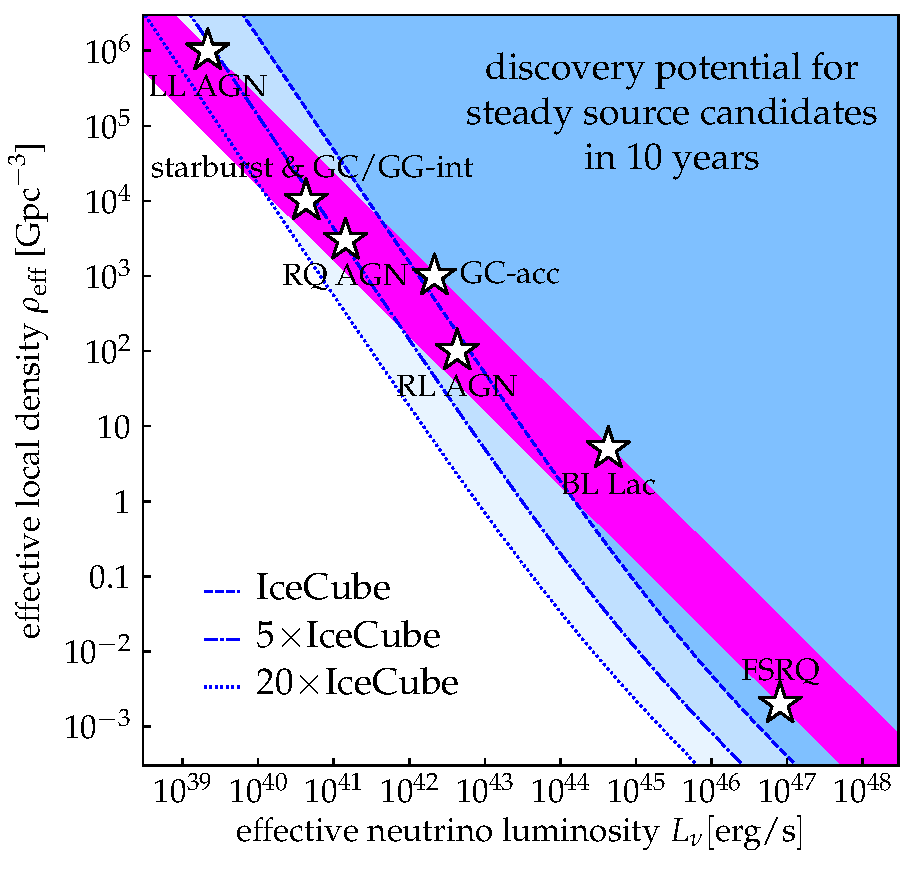
\includegraphics[width=0.45\linewidth]{img/sources_steady.pdf}
    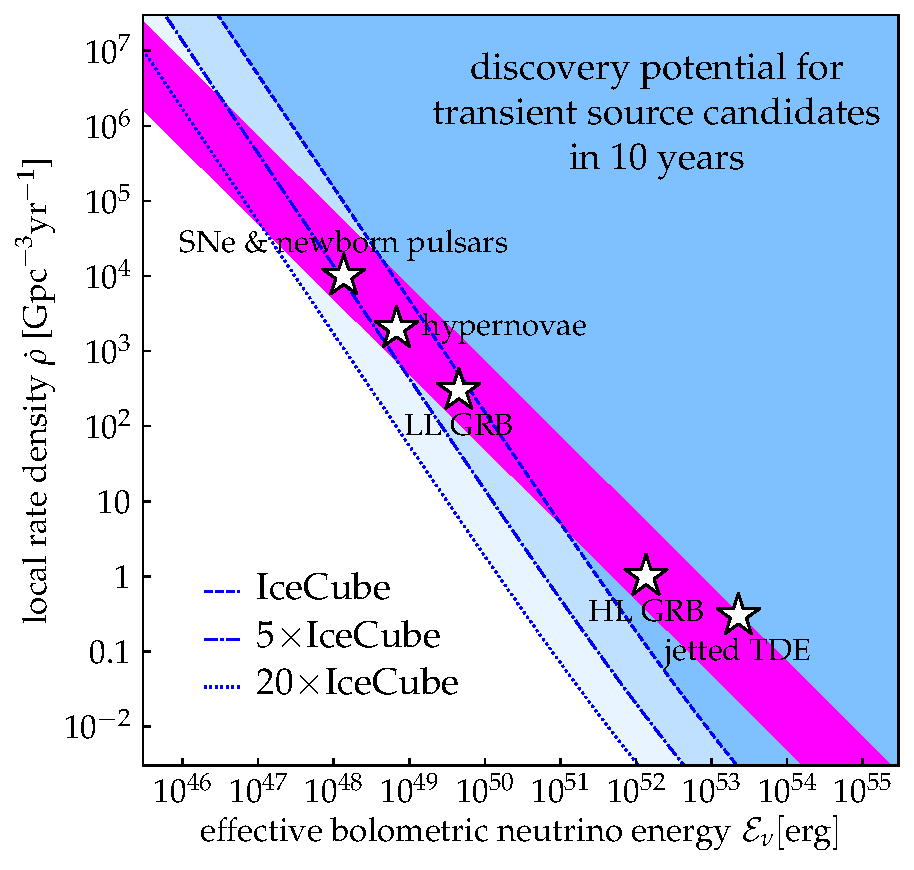
\includegraphics[width=0.45\linewidth]{img/sources_transient.pdf}
    \caption{IceCube观测对天体物理中微子源的限制。左侧:观测到的弥散中微子流量(洋红色带状区域)和天体物理源持续源的密度以及光度的关系。洋红色带状的宽度表示源的红移演化的不确定性。蓝色阴影区域表示IceCube以10年观测数据的探测能力(discover potential)。一些可能的天体物理源用白色星星标记了出来。右侧:IceCube探测能力与暂现源的事例率以及爆发能量之间的关系。图片来自\cite{Astro2020_neutrino}}
    \label{fig:neutrino_sources}
\end{figure}

\subsubsection{高能天体中微子源的搜寻}

IceCube根据不同的数据样本进行过大量地对中微子源的搜索尝试。例如IceCube使用来自全天的径迹型事件来搜索中微子的点源\cite{IceCube_10yr_point_source:2019},其数据分析得到的热点图如图\ref{fig:IceCube_10yr_source_hotspot}所示。
除了径迹型事件以外,IceCube还使用簇射型事件来搜索中微子点源\cite{IceCube_7yr_cascade_source:2019},这些事件在南天拥有更好的灵敏度。

\begin{figure}[htbp]
    \centering
    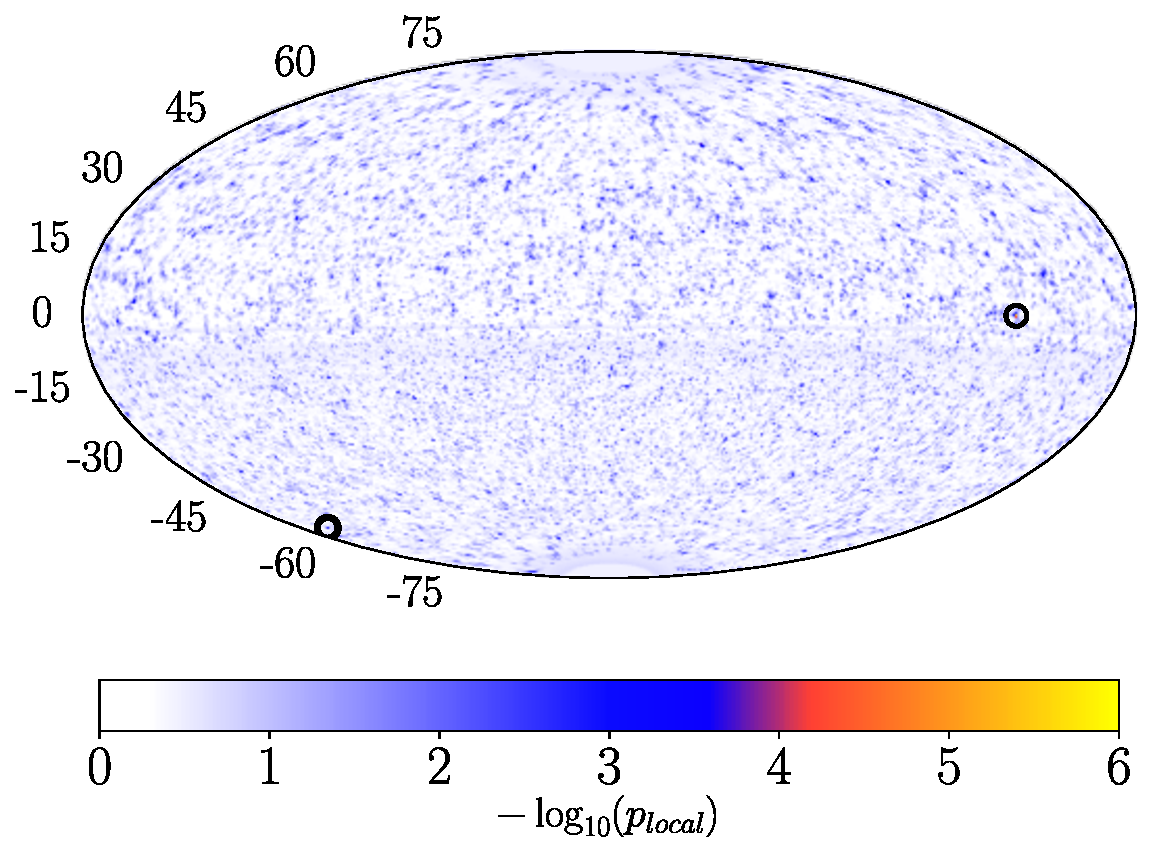
\includegraphics[width=0.6\linewidth]{img/IceCube_10yr_source_hotspot.pdf}
    \caption{IceCube对10年径迹型事件分析得到的中微子源的热点图。上下两个黑圈分别表示北天和南天最显著的源,分别是NGC 1068和PKS 2233-148。图片来自\cite{IceCube_10yr_point_source:2019}}
    \label{fig:IceCube_10yr_source_hotspot}
\end{figure}

通过对全天搜索得到的中微子源热点进行进一步的分析,IceCube发现了NGC 1068可能是一个中微子源\cite{IceCube_NGC1068:2022}。NGC 1068是一个距离地球仅为$14\,\mathrm{Mpc}$的Seyfert II型星系,它的中心有一颗被尘埃掩盖的超大质量黑洞\cite{Rosas_NGC_1068:2021}并且还是一个星爆星系。IceCube通过对径迹型事件进行分析,以$4.2\sigma$的置信度确认了NGC 1068是一个中微子源,其最佳拟合的中微子流量能谱如下:
\begin{equation}
\begin{aligned}
    \phi^{\nu_\mu+\bar{\nu}_\mu}(E_\nu) &= 
    \phi^{\nu_\mu+\bar{\nu}_\mu}_\mathrm{1\,TeV} 
    \times \left( \frac{E_\nu}{1\,\mathrm{TeV}} \right)^{-\gamma} 
    \times 10^{-11} \, \mathrm{s^{-1} cm^{-2} TeV^{-1}}, \\
    \phi^{\nu_\mu+\bar{\nu}_\mu}_\mathrm{1\,TeV} &= 
    5.0 \pm 1.5_\mathrm{stat} \pm 0.6_\mathrm{sys}, ~~
    \gamma = 3.2 \pm 0.2
    \label{eq:spectrum_NGC1068}
\end{aligned}
\end{equation}

对于实时暂现源的研究,IceCube设计了一套实时的多信使预警系统\cite{IceCube_alert:2016, IceCube_alert:2019},可以快速发布它观测到的高质量的中微子信号。
对于其他设备的观测结果,例如伽马射线和引力波等,IceCube中也存在一套跟随观测系统\cite{IceCube_follow_up:2020}用于快速发布可能的关联中微子信号或者给出中微子流量的上限。

2017年,IceCube观测到了一个约$270\,\mathrm{TeV}$的高能径迹型中微子事件(IceCube-170922A),该中微子事件与一个Fermi的耀变体数据库中的一个正在活跃期的耀变体TXS 0506+056在时间和空间上成协\cite{TXS_0506_MM:2018}。
而且通过对该方向上的中微子流量进行历史上的追溯搜索,IceCube发现该耀变体在2015年期间还有一次大规模的中微子流量超出,其置信度达到了$3.5\sigma$\cite{TXS_0506_flare:2018}。
这是人们首次成功地通过高能中微子事件来进行多信使观测,它打开了高能中微子多信使研究的大门。

除了对全天弥散的中微子流量进行点源搜寻以及通过实时多信使事件来搜寻暂现源,IceCube还对各种不同类别的中微子源进行了系统性的分类搜寻,其搜寻的分析和结果如下:

\begin{enumerate}
    \item \textbf{伽马射线暴}。IceCube对Fermi库中的GRB进行了时空上的成协分析,表明来自Fermi库中的GRB所产生的中微子辐射最多只能占弥散中微子流的$\sim 1\%$\cite{IceCube_GRB_prompt:2014, IceCube_GRB:2022}。尽管如此,来自低光度GRB和喷流被束缚的GRB(choked jet GRB)\cite{Choked_GRB:2015}对中微子流量的贡献依然无法被限制。

    \item \textbf{活动星系核和耀变体}。Fermi-2LAC的耀变体(blazar)样本与中微子的成协分析表明,这些耀变体最多贡献弥散中微子流的27\%。\cite{IceCube_Fermi_2LAC_blazars:2016}。另一项工作采用了不同的AGN样本,他们通过对软X射线辐射较强的AGN来进行相关性分析,然后也没有得到很高的置信度($2.6\sigma$)\cite{IceCube_AGN_core:2021}。

    \item \textbf{河内中微子源}。对于来自银河系内的中微子辐射,IceCube的分析表明其对弥散中微子流的贡献小于14\%\cite{IceCube_galactic:2017}。IceCube和ANTARES对银盘中微子流的联合分析没有找到明显的超出\cite{ANTARES_IceCube_galactic:2018}。IceCube对PWN和X射线双星的分析中都没有找到成协的源\cite{IceCube_PWN:2020, IceCube_X_binaries:2022}。IceCube中微子与HAWC\cite{IceCube_HAWC:2019}和LHAASO\cite{Huang_IceCube_LHAASO:2021, IceCube_LHAASO:2022}的高能伽马射线源的联合分析也没有找到中微子信号的超出。

    \item \textbf{快速射电暴}。IceCube对快速射电暴(Fast Radio Burst,FRB)样本进行过多次的时间和空间相关联的中微子信号寻找\cite{IceCube_FRB:2017, IceCube_FRB:2019, IceCube_FRB:2022},但都没有找到相关联的信号。

    \item \textbf{双致密星并合}。IceCube对LIGO-Virgo探测到的双致密星并合事件做过一些关联性分析\cite{GW170817_MM, IceCube_ANTARES_Auger_GW170817, IceCube_BBH:2020},分析中并没有找到中微子信号超出。

    \item \textbf{潮汐瓦解事件}。目前光学望远镜已经发现了3个与IceCube中微子信号在时间和空间上成协的的TDE事件\cite{TDE_MM:2023}:AT2019dsg\cite{AT2019dsg:2020},AT2019fdr\cite{AT2019fdr:2021}和AT2019aalc,而IceCube合作组尚未发表有关TDE和中微子信号的分析文章。

\end{enumerate}


\subsubsection{味道分辨}

来自天体物理源的高能中微子的味道测量对于研究中微子源内发生的物理过程以及寻找新物理有重要的意义\cite{Arguelles_flavor:2015, snowmass_flavor:2022}。根据标准模型的预言,在源处发射的味道为$\alpha$的中微子在经过超长基线振荡后转变为$\beta$味道的中微子的几率为\cite{Farzan_coherence_oscillation:2008}:
\begin{equation}
    \left\langle P_{\nu_\alpha \rightarrow v_\beta}\right\rangle=\sum_i\left|U_{\alpha i}\right|^2\left|U_{\beta i}\right|^2, 
    \label{eq:flavor_transform}
\end{equation}
其中$U$为公式\ref{eq: neutrino oscillation}中介绍的PMNS矩阵。

在假设中微子源处的味道比例为$\nu_e: \nu_\mu: \nu_\tau=1 / 3: 2 / 3: 0$,那么在地球中观测到的中微子的味道比例就应该是$\nu_e: \nu_\mu: \nu_\tau = 0.30 : 0.36 : 0.34$,与$1/3 : 1/3 : 1/3$相接近。
而在假设一些超出标准模型的效应,例如惰性中微子\cite{IceCube_sterile:2016, Arguelles_flavor_sterile:2019},洛伦兹对称性破缺\cite{IceCube_flavor_Lorentz:2017}等的情况下,地球上观测到的中微子味道的比例可能会与$1/3 : 1/3 : 1/3$发生强烈的偏离。

长期以来,IceCube都在从观测到的高能中微子数据中中微子味道比例\cite{IceCube_flux_flavor:2015, IceCube_inelestic_flavor:2018, IceCube_tau:2020}。
图\ref{fig:IceCube_flavor_ratio_measurement}展示了IceCube最新的测量结果。

\begin{figure}[htbp]
    \centering
    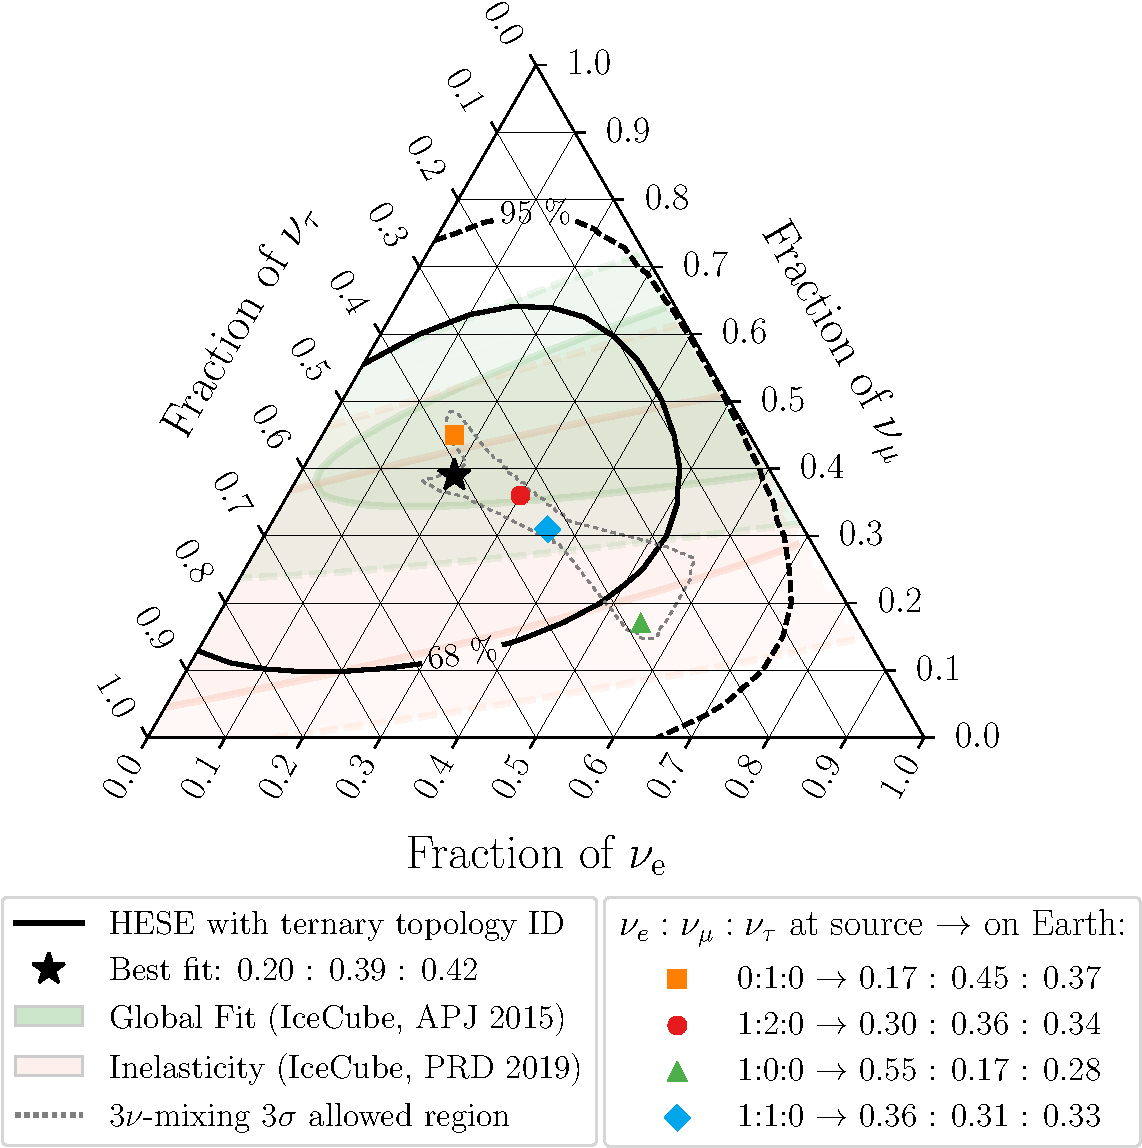
\includegraphics[width=0.9\linewidth]{img/IceCube_flavor_ratio_measurement.pdf}
    \caption{IceCube对中微子味道的测量结果以及理论预测值。途中的黑线\cite{IceCube_tau:2020},绿色阴影区域\cite{IceCube_flux_flavor:2015},粉色区域\cite{IceCube_inelestic_flavor:2018}分别表示IceCube三次用不同的方法实现的中微子味道的测量结果。实心的正方形,圆形,三角形,棱形分别表示几种典型的源处中微子味道比例所对应的地球上理论预期的比例。图片来自\cite{IceCube_tau:2020}}
    \label{fig:IceCube_flavor_ratio_measurement}
\end{figure}
